\section{Improving forecasts with history}
\label{sec:nw_hist_model}

The model presented in \cref{sec:nw_model,sec:nw_realtime,sec:nw_par_est} is adequate for estimating the \emph{real-time} state of the network, but is unuseful for forecasting vehicle speeds, particularly just before or after a peak period. In \cref{cha:prediction}, we explore the prediction of arrival times, which involves making short-term forecasts of speed. Using historical data is one way of improving speed forecasts, particularly around peak times.


In \cref{nw_par_est_real}, I showed that most roads have a ``peak effect'' in the morning or the evening, while some exhibit both. It seems reasonable therefore to have a model which allows a segment to have zero, one, or two peaks, each with varying magnitude (the size of the decrease in speed) and width (how long the peak period is). The temporal location of these peaks is likely to be related, but variable: some roads will experience peak traffic earlier than others, for example.

\begin{knitrout}\small
\definecolor{shadecolor}{rgb}{0.969, 0.969, 0.969}\color{fgcolor}\begin{figure}

{\centering 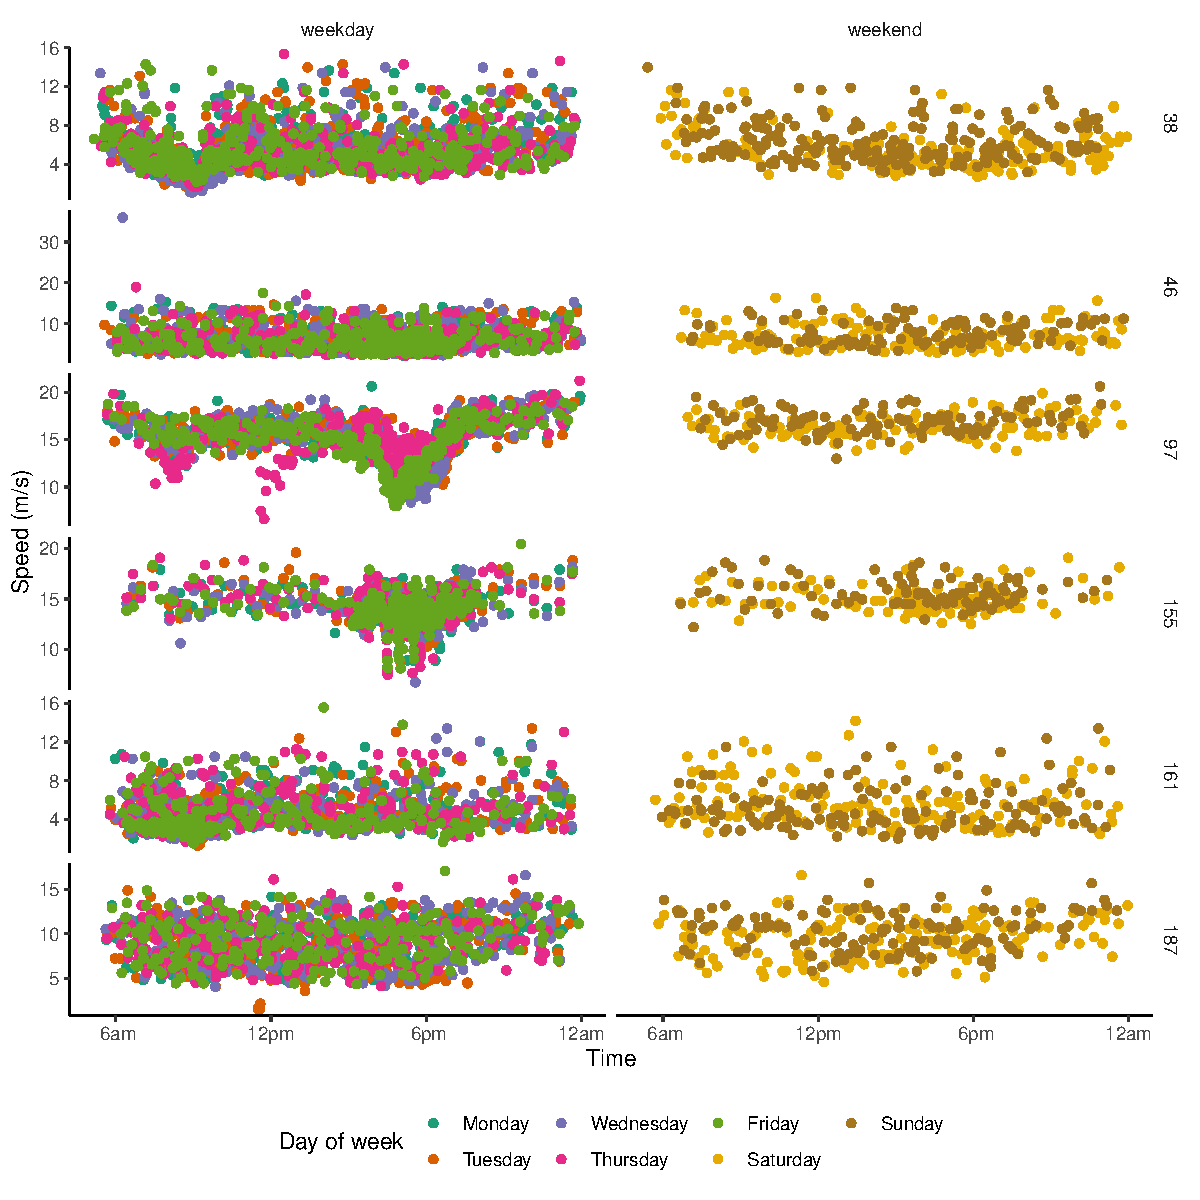
\includegraphics[width=\textwidth]{figure/tt_week0_load-1} 

}

\caption[Vehicle speeds along six road segments over one week]{Vehicle speeds along six road segments over one week, coloured by the day of the week.}\label{fig:tt_week0_load}
\end{figure}


\end{knitrout}

Early work fitting Bayesian models to these data were not promising, as it involved too much manual work tuning the parameters for each segment and checking the results. Since our goal is to obtain a generalised framework that runs with minimal manual effort, we sought an alternative.

From \cref{fig:tt_week0_load} it is clear that along each segment, there is a consistent pattern, with some variability between days as far as the temporal location and magnitude of the ``peak'' on weekdays; weekends are fairly consistent, although this is only two days' worth of data. Here I present a nearest-neighbour grid, which takes time and road state (traffic speed) as input, and outputs the mean (and uncertainty) of travel time in 10, 20, or 30~minutes from the current time. Similar ``speed maps'' have been used by the likes of \citet{Cathey_2003, Celan_2017, Chen_2014}. The first step is to aggregate observations into 5~minute intervals and take the mean traffic speed in each interval. Next, we bind lagged duplicates of these speeds (10, 20, 30~minutes, for example), such that each row includes current and future states. Any missing periods are interpolated from the mean of the adjacent states. The speed map for 30~minute predictions is shown in \cref{fig:tt_week0_grid}. The lighter areas represent higher speeds.







\begin{knitrout}\small
\definecolor{shadecolor}{rgb}{0.969, 0.969, 0.969}\color{fgcolor}\begin{figure}

{\centering 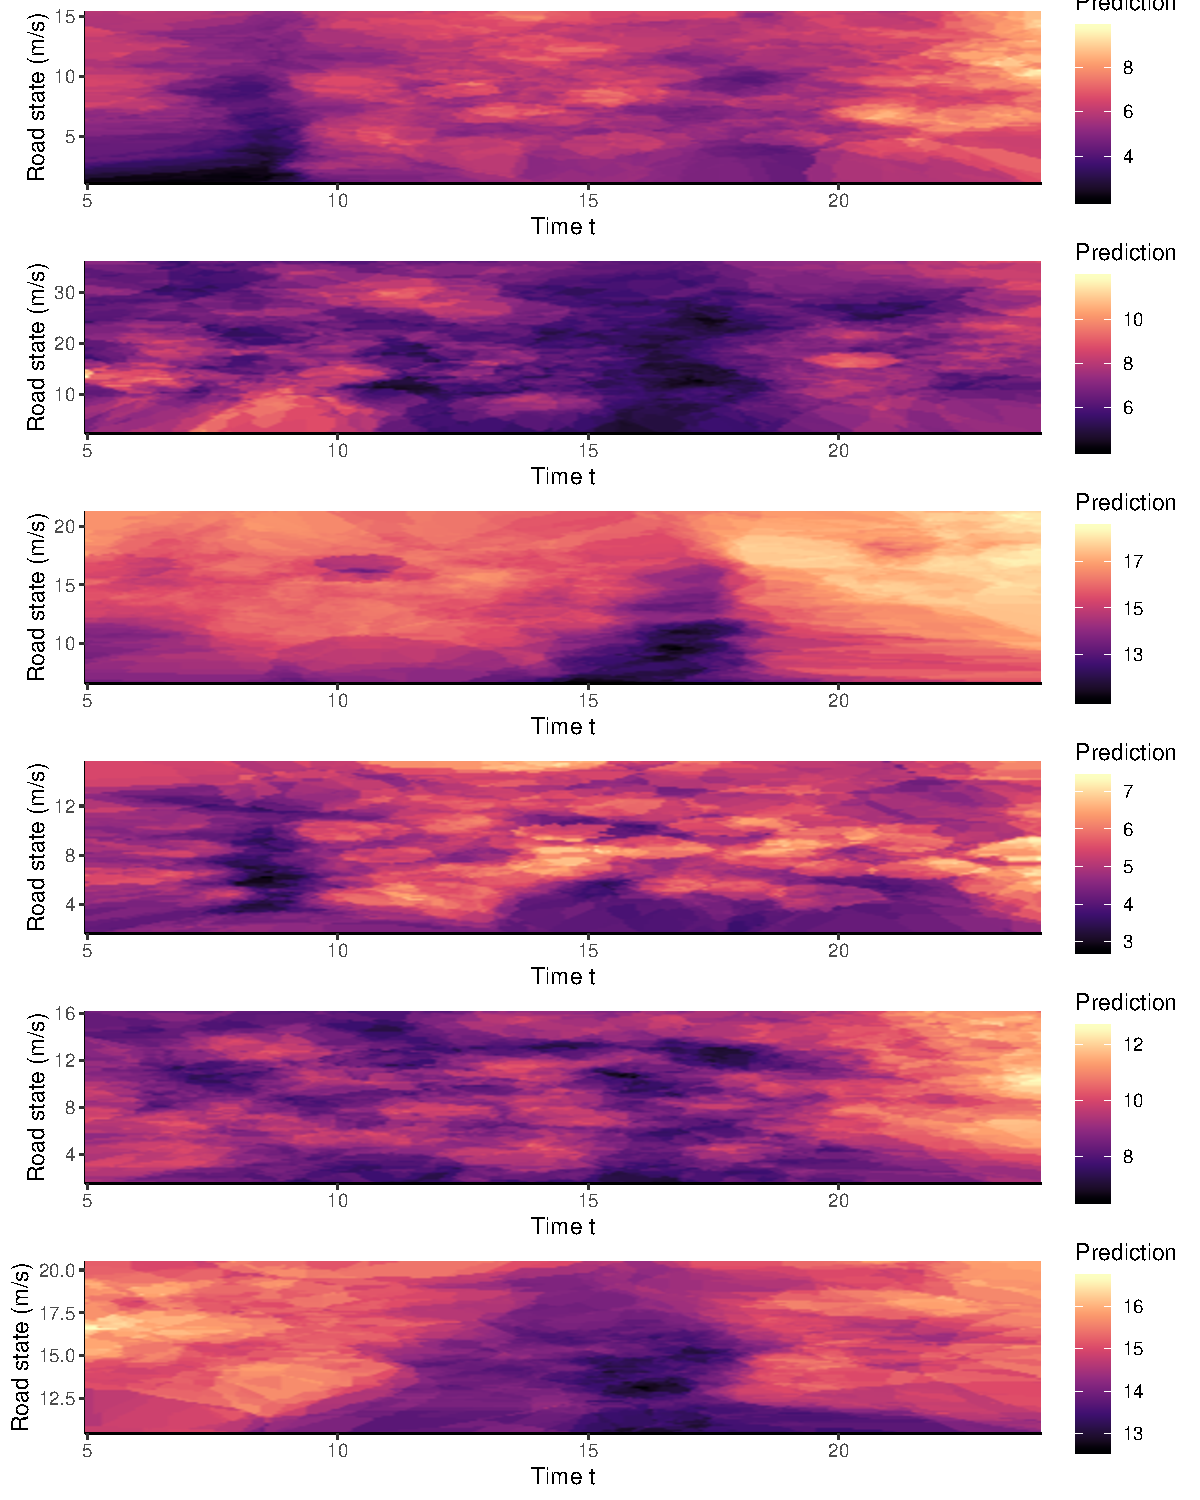
\includegraphics[width=\linewidth]{figure/tt_week0_grid-1} 

}

\caption[Speed maps to predict segment speed in 30~minutes given the current state]{Speed maps to predict segment speed in 30~minutes given the current average speed (y-axis) and time (x-axis).}\label{fig:tt_week0_grid}
\end{figure}


\end{knitrout}

The next step is to evaluate the predictive power of this approach. We do this by taking the second week of data (shown in \cref{fig:tt_week1_load}) and use the fitted estimates to predict the state in 30~minutes, and then compare this to the actual state in 30~minutes. The \gls{rmse} (\cref{app:error-functions}) is used to compare the predicted and observed speeds.



\begin{knitrout}\small
\definecolor{shadecolor}{rgb}{0.969, 0.969, 0.969}\color{fgcolor}\begin{figure}

{\centering 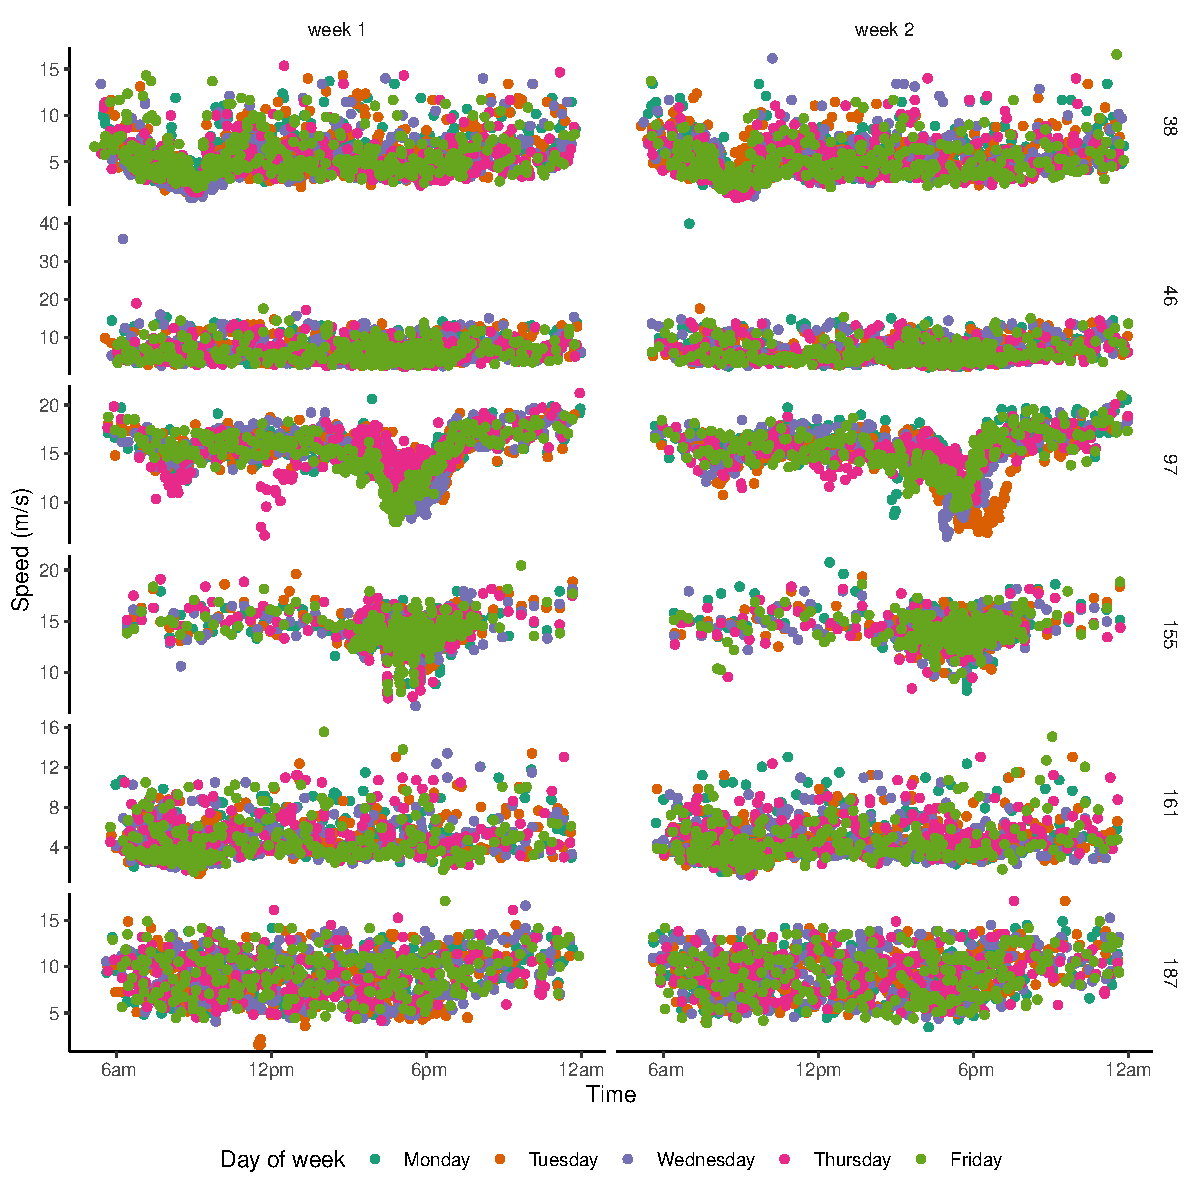
\includegraphics[width=\linewidth]{figure/tt_week1_load-1} 

}

\caption[Vehicle speeds along six roads over of two weeks.]{Vehicle speeds along six roads over the course of two weeks, showing only week days, for training (left) and testing (right).}\label{fig:tt_week1_load}
\end{figure}


\end{knitrout}

\begin{knitrout}\small
\definecolor{shadecolor}{rgb}{0.969, 0.969, 0.969}\color{fgcolor}\begin{figure}

{\centering 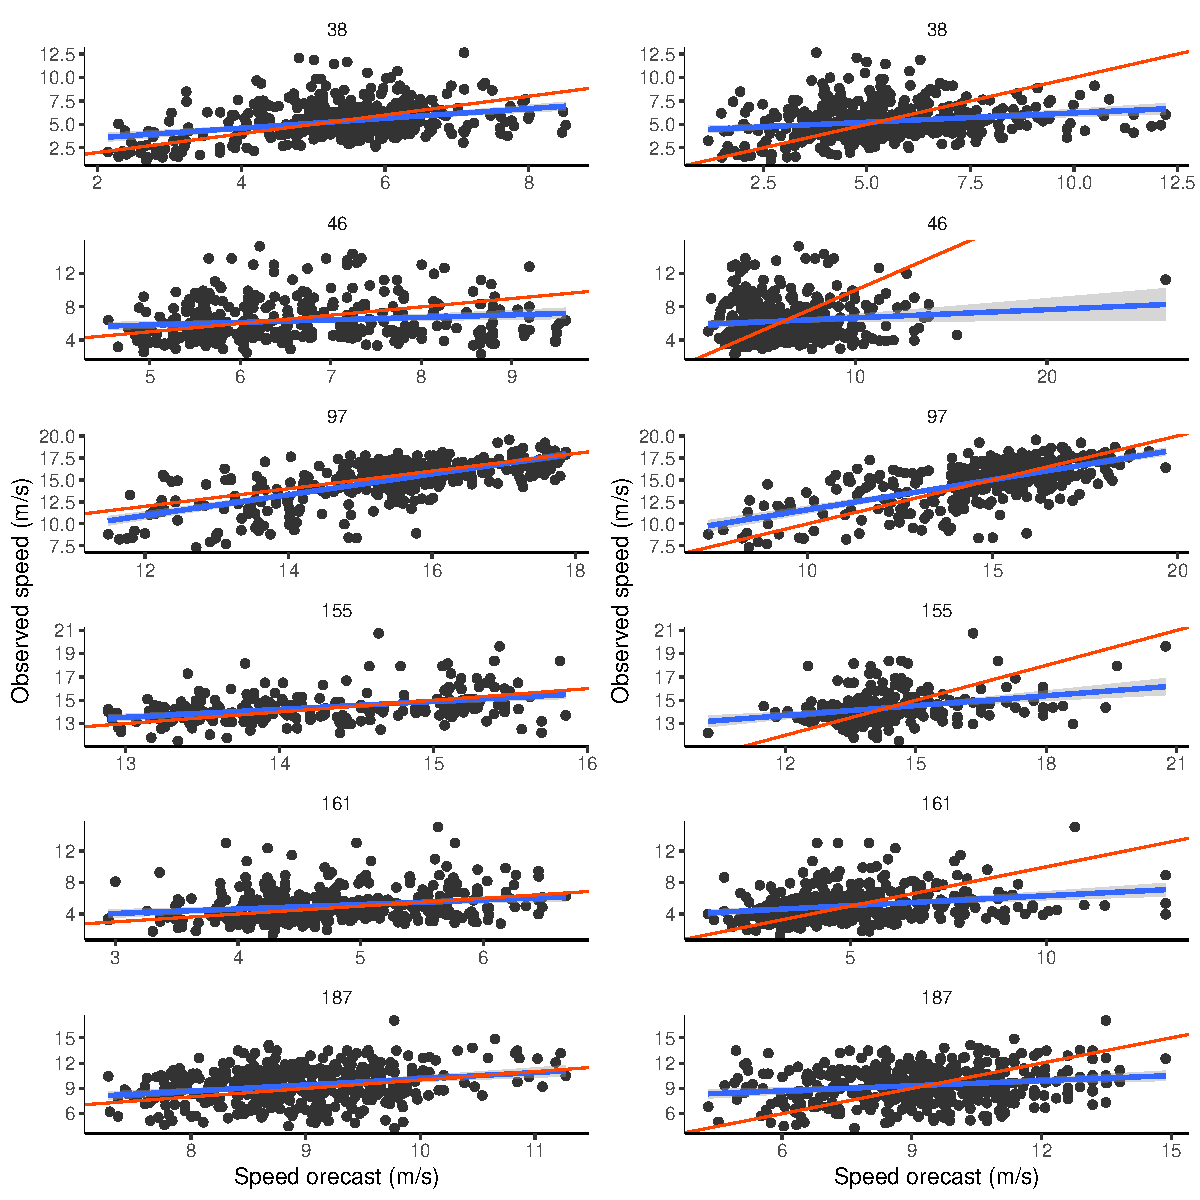
\includegraphics[width=\linewidth]{figure/tt_week1_pred-1} 

}

\caption[Forecasts of average vehicle speeds in 30 minutes versus actual average speed in 30 minutes along segments]{Forecasts of average vehicle speeds in 30 minutes versus actual average speed in 30 minutes along segments. The line of equality (red) indicates a perfect prediction. The closer the best fit line (blue) is to the line of equality, the better the forecasts.}\label{fig:tt_week1_pred}
\end{figure}


\end{knitrout}


Forecasts 30~minutes into the future are shown in \cref{fig:tt_week1_pred} for both the grid-search method, as well as the na\"ive method of using the current average traffic speed as the predictor. The comparative \gls{rmse} values are displayed in \cref{tab:tt_pred_rmse}. However, these are not too different because there is a lot of inherent uncertainty, but demonstrate a slight increase in predictive performance when historical trends are used.


Most importantly, however, is the linear curve (shown in blue in \cref{fig:tt_week1_pred}) compared to the line of equality, in red. The interpretation is that the more accurate the predictions on average, the closer the blue trend line will be to the black line of equality. For our forecast model, we see that in 5 out of 6 segments the two lines are very close, compared to the na\"ive estimate in which case the predictions are often too high or too low.


Further work is needed to improve the forecasting abilities of our model. However, we have designed the framework in such a way that any such improvements can easily be integrated into both the network modelling stage, and the upcoming arrival time prediction stage (see \cref{sec:nw_implementation_forecast} for details).

\begin{table}

\caption{\label{tab:tt_pred_rmse}RMSE results comparing the predictive performance of two forecast methods for predicting road state in 30~minutes.}
\centering
\begin{tabular}[t]{lr}
\toprule
Method & RMSE (m/s)\\
\midrule
Simple & 2.48\\
Forecast & 1.99\\
\bottomrule
\end{tabular}
\end{table}


